\chapter{LLVM}
\section{History}
\begin{wrapfigure}{l}{.5\textwidth}
    \caption[The logo of LLVM]{The logo of LLVM \cite{llvmLogo}}
    
\includegraphics[width=.5\textwidth]{gfx/llvmLogo.png}
\end{wrapfigure}
\llvm is a collection of modular and reusable compiler and toolchain technologies to support static and dynamic compilation as well as transparent and lifelong program analysis and transformations of arbitrary programs. \cite{LLVMWebsite, LLVMResearchBeginning}\\
Former \llvm has been a reasearch project at the university of Illinois, which was first described in a publication in 2004.
The project has grown so popular that in 2014 the LLVM Foundation was founded for organizing and maintaining the project. \cite{LLVMFoundation}\\
The main goal of \llvm consists of the creation of a compiler framework in which the optimizations and analysis are independent from the underlying os and the used programming language.
To archive the independency \llvmir was created which is solely used within the pipeline.
\enquote{\llvmir is a strongly typed, \ac{SSA} language that connects to a wide variety of high-level languages.} \cite{PolyhedralEmpiricalStudy}

\section{Pipeline}
The \llvmir, on which the components operate, is generated when entering the pipeline of \llvm (\autoref{fig:llvmPipeline}) by translating the files containing sourcecode written in an arbitrary programming language using a frontend like clang.
When leaving the pipeline files containing the appropriate assembler instructions are created out of the (possibly) newly formed \llvmir by the \generator. \cite{IntroLLVM}
\begin{figure}[!ht]
    \caption{The pipeline of LLVM}
    \label{fig:llvmPipeline}
    \centering
    \begin{tikzpicture}
        \node(languages)[nonLlvmIrNode, align=center]{C/C++, Obj-C,\\Python, Ruby,...};
        \node(frontend)[nonLlvmIrNode, right=of languages]{compiler frontend};
        \node(opt1)[llvmIrNode, right=of frontend]{\opt};
        \node(llvmLinker)[llvmIrNode, below=of opt1]{\linker};
        \node(opt2)[llvmIrNode, below=of llvmLinker]{\opt};
        \node(generator)[llvmIrNode, left=of opt2]{\generator};
        \node(linker)[nonLlvmIrNode, left=of generator]{System Linker};
        \path[nonLlvmIrPath] (languages) to (frontend);
        \path[llvmIrPath] (frontend) to (opt1);
        \path[llvmIrPath] (opt1) -| ($(opt1.north east) + (0.5,0.5)$) -| node[auto]{Pass} (opt1);
        \path[llvmIrPath] (opt2) -| ($(opt2.south east) + (0.5,-0.5)$) -| node[auto]{Pass} (opt2);
        \path[llvmIrPath] (opt1) to (llvmLinker);
        \path[llvmIrPath] (llvmLinker) to (opt2);
        \path[llvmIrPath] (opt2) to (generator);
        \path[nonLlvmIrPath] (generator) to (linker);
    \end{tikzpicture}
    \legend
\end{figure}\\
\subsection{compiler frontend}\label{subsec:compilerfrontend}
So the first step at the beginning of the pipeline is translating the files containing sourcecode by a front end like the clang (C, C++, Objective-C), Fortran (llvm-gfortran), Python (PyLLVM) \draftnote{cite?}, Ruby (llvmRuby) \draftnote{Still existing?}, Java (IcedTea) and .NET (IcedTea?!) \draftnote{cite GrosserDiploma}.
From now on this work is only discussing clang as frontend. \draftnote{Schöner formulieren}
Using clang \llvmir can be generated by adding the option \texttt{-emit-llvm} in order \enquote{to abstract away from the specifics} \cite{FastScopDetection} of a programming language.
The option \texttt{-S} may also be passed to generate a human readable textfile instead of a \llvmir binary.
\subsection{LLVM Optimizer}\label{subsec:optimizer}
On these files the the \opt can perform steps for optimizing and analysing the code.
These steps are called \enquote{Passes}.
Such passes are be explicitly invoked by appending the appropriate options to the command \texttt{opt} of the the \opt and can be applied to the single files or to the already linked program.
It is also possible to add further custom options by loading (multiple) libraries using the flag \texttt{-load}.
When calling the the \opt the option \texttt{-S} may also be specified for generating a human readable textfile similar to clang in \autoref{subsec:compilerfrontend}.
\subsection{LLVM Linker}
The \linker links the optimized \llvmir files and applies further optimizations.
\subsection{LLVM Code Generator}
When all desired passes are performed the \generator translates \llvmir into target assembler.
\subsection{Control Flow Graph (CFG)}
\begin{wrapfigure}{l}{.3\textwidth}
    \caption{The CFG of \autoref{lst:matmulll}}
    \label{fig:exampleCfg}
    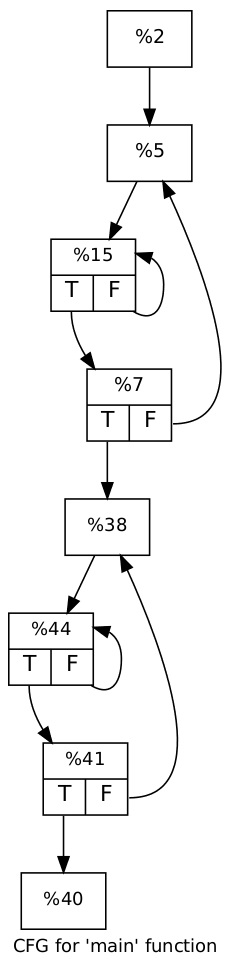
\includegraphics[height=12cm]{gfx/matmulCfg.png}
\end{wrapfigure}
At any point the current \cfg of a \llvmir file can be visualized (like \autoref{fig:exampleCfg}) by passing one of the options \texttt{-view-cfg} or \texttt{-view-cfg-only} to the the \opt.
The \cfg is used by many analysis and optimization passes for determining which optimizations can or should be applied.
